% !TeX root = ../libro.tex
% !TeX encoding = utf8
\chapter{Arquitectura Software}
\section{Introducción}
En el desarrollo de aplicaciones, la arquitectura subyacente puede definir tanto su funcionalidad como su escalabilidad. A continuación, veremos los principales tipos de arquitecturas que suelen utilizar las aplicaciones hoy en día. Mencionaremos las ventajas e inconvenientes que tienen cada una de ellas, con el fin de saber cuál es la que mejor se adapta a cada aplicación según las necesidades del proyecto. 

Vamos a estudiar las arquitecturas monolíticas, cliente-servidor, basadas en microservicios, y posteriormente veremos la Arquitectura Orientada a Servicios (\textit{Service Oriented Architectures, SOA}) junto con el modelo REST (Transferencia de Estado Representacional) y su implementación en las aplicaciones, conocida como RESTful.
\section{Arquitectura de una aplicación}
La arquitectura de una aplicación describe cómo encajan sus piezas a alto nivel. Los desarrolladores utilizan muchos tipos de arquitecturas. Muchas de estas abordan características particulares del problema que se está resolviendo.

Por ejemplo, los sistemas basados en reglas se suelen utilizar para manejar situaciones complejas, en las que resolver un problema particular se pueda reducir a seguir un conjunto de reglas. Algunos sistemas de resolución de problemas utilizan este enfoque.
Algunas de las arquitecturas que veremos son:
\begin{itemize}
	\item Monolítica. Todas las funciones de la aplicación se implementan en un solo programa, lo que puede simplificar el desarrollo pero limita la flexibilidad y escalabilidad a medida que la aplicación crece.
	\item La arquitectura cliente-servidor separa las funciones de la aplicación en dos partes distintas: el cliente, que es la interfaz de usuario, y el servidor, que maneja el procesamiento y el almacenamiento de datos. Esta separación permite una mayor escalabilidad y distribución de tareas, pero puede introducir complejidad adicional en la comunicación entre el cliente y el servidor.
	\item La arquitectura orientada a servicios (SOA) es un enfoque en el que las diferentes funciones de la aplicación se exponen como servicios independientes, lo que permite una mayor reutilización y flexibilidad en el desarrollo de software empresarial.
	\item Arquitectura de microservicios. No son sólo un tipo de arquitectura, sino también un modo de abordar la escritura del software. Con ellos, las aplicaciones se dividen en sus elementos más pequeños, que son independientes entre sí. Cada uno de dichos elementos o procesos es un microservicio.
	\item REST es un estilo arquitectónico para diseñar sistemas distribuidos que se basa en la idea de que cada recurso se identifica mediante un URI y se puede acceder y manipular a través de operaciones estándar de HTTP como GET, POST, PUT y DELETE. Esta arquitectura es especialmente adecuada para aplicaciones web y servicios web que requieren una alta escalabilidad y rendimiento.
\end{itemize}

En resumen, cada tipo de arquitectura tiene sus propias ventajas y desventajas, y la elección de la arquitectura depende por tanto de los requisitos y las restricciones específicas de cada proyecto.
\subsection{Arquitectura monolítica}
En una arquitectura monolítica, un solo programa hace todo. Muestra la interfaz de usuario, accede a los datos, procesa cualquier petición del servidor y hace todo lo que la aplicación necesite.

Esta arquitectura tiene algunas desventajas significativas. En particular, las piezas del sistema están estrechamente vinculadas, por lo que no te ofrece mucha flexibilidad.

Una arquitectura monolítica también requiere comprender cómo encajan todas las piezas del sistema desde el principio del proyecto. Si se comete algún error en los detalles, el acoplamiento estrecho entre las piezas del sistema dificulta corregirlos más tarde.
Sin embargo, las arquitecturas monolíticas tienen algunas ventajas, debido a que todo está integrado en un solo programa, no es necesario tener una comunicación complicada a través de redes.
Las arquitecturas monolíticas también son útiles para aplicaciones pequeñas donde un solo programador o equipo está trabajando en el código.\\

Dos ejemplos de arquitecturas monolíticas muy popularizados son los ERP (Enterprise Resource Planning), son una forma de dar lógica a las enormes cantidades de datos dentro de una organización y permitir el flujo de información entre los diferentes equipos de manera automática y sin inconvenientes, y los CRM (Customer Relation Management).

La información que hemos obtenido para describir la arquitectura monolítica está basada en \cite{stephens2015beginning}.
\subsection{Cliente-Servidor}
Una arquitectura cliente-servidor separa las piezas del sistema que necesitan usar una función particular (clientes) de las partes del sistema que proporcionan esas funciones (servidores). Eso desacopla las piezas de cliente y servidor del sistema para que los desarrolladores puedan trabajar en ellas por separado.
Por ejemplo, muchas aplicaciones dependen de una base de datos para mantener información, y la aplicación necesitará mostrar esa información en algún tipo de interfaz de usuario. Una forma de hacerlo sería integrar la base de datos directamente en la aplicación.
Un problema con este diseño es que múltiples usuarios no pueden usar los mismos datos. Este problema se puede solucionar pasando a una arquitectura de dos niveles donde un cliente (la interfaz de usuario) está separado del servidor (la base de datos). Los clientes y el servidor se comunican a través de alguna red como una red de área local (LAN), red de área amplia (WAN) o Internet.
\begin{figure}[h!]
	\centering
	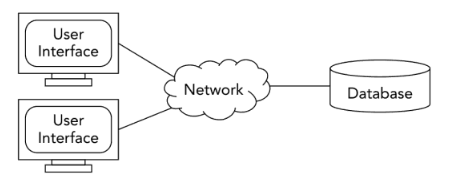
\includegraphics[width=0.8\textwidth]{2niveles}
	\caption{Arquitectura de $2$ niveles, donde el cliente está separado del servidor}
	\label{fig:2niveles}
\end{figure}
La arquitectura de dos niveles facilita el soporte de múltiples clientes con el mismo servidor, pero vincula estrechamente a clientes y servidores. Los clientes deben saber qué formato utiliza el servidor, y si se cambia la forma en que el servidor presenta sus datos, se necesita también cambiar el cliente para que coincida. Eso puede suponer un trabajo extra, especialmente al principio de un proyecto cuando las necesidades del cliente y del servidor no están completamente definidas. Podemos ver una imagen de la arquitectura de dos niveles en la \autoref{fig:2niveles}.

Otra opción es aumentar la separación entre los clientes y el servidor introduciendo otra capa entre los dos para crear una arquitectura de tres niveles.
En este caso, el nivel intermedio proporciona una separación entre los clientes y el servidor, la cual permite que diferentes equipos trabajen sin interferir demasiado entre sí.
Además de proporcionar separación, un nivel intermedio puede realizar otras acciones que hagan que los datos sean más fáciles de usar tanto para el cliente como para el servidor.

Se pueden definir otras arquitecturas multinivel que utilicen más de tres niveles si fuera necesario. Por ejemplo, un nivel de datos podría almacenar los datos, un segundo nivel podría calcular agregaciones y realizar otros cálculos sobre los datos, un tercer nivel podría usar técnicas de inteligencia artificial para hacer recomendaciones basadas en los datos del segundo nivel, y un cuarto nivel sería de presentación que permitiría a los usuarios ver los resultados.\\

Algunos ejemplos de aplicaciones actuales que utilizan la arquitectura cliente-servidor son:
\begin{itemize}
	\item \textit{Outlook} es un cliente de correo que sirve para leer los correos del servicio \textit{hotmail}.
	\item \textit{WhatsApp} o \textit{Telegram} son clientes de servicios de chat, video, audio...
	\item \textit{Firefox} es un cliente web, \textit{Chrome} también, son navegadores.
\end{itemize}

La información que hemos obtenido para describir la arquitectura cliente-servidor está basada en \cite{stephens2015beginning}.
\subsection{Arquitectura Orientada a Servicios, SOA}
En los últimos años, SOA ha recibido una atención creciente en línea con el movimiento hacia abordar los desafíos asociados con la mejora y mantenimiento de diversos entornos. Con el objetivo de modernizar el sistema de software de las organizaciones, la migración de un sistema heredado a un sistema basado en SOA se ha convertido en una tendencia predominante. \\
Son varios los beneficios de emplear SOA en el desarrollo de tecnologías líderes en el mundo actual, como \textit{Internet of Things} (IoT) y \textit{Cloud Computing} (CC), además de microservicios. Esto se debe a que SOA ofrece integración flexible y reutilización de servicios debido a su arquitectura modular basada en servicios. SOA también ofrece transparencia porque encapsula varias aplicaciones y fuentes de datos en forma de caja negra. De esta manera, un conjunto integrado de recursos de Tecnologías de la Información (TI) aún podría ser accesible a pesar de la existencia de diversas tecnologías, códigos de lenguaje, funcionalidades y plataformas.

Aunque no hay una definición clara de SOA, en \cite{soa} se define como un concepto arquitectónico que promueve el acoplamiento flexible, la reutilización, la interoperabilidad, la agilidad, la eficiencia, con un enfoque en descomponer cada proceso empresarial en bloques más pequeños de tareas y funciones como servicios. Estos servicios están bien definidos y organizados y sirven como unidades independientes de funcionalidad empresarial estándar que están conectadas entre sí para crear un proceso empresarial unificado.

En \cite{soa} se indican varios estudios que afirman que la combinación de SOA con otras tecnologías podría proporcionar más beneficios para las organizaciones. Podría integrarse con nuevas tecnologías médicas, agentes inteligentes, tecnologías inalámbricas, identificación por radiofrecuencia (RFID) y procedimientos operativos de Internet para establecer nuevas automatizaciones para el proceso empresarial. Además, los requisitos de IoT podrían cumplirse mediante el enfoque SOA, ya que puede proporcionar medición de rendimiento, detección de ataques de seguridad e inteligencia empresarial.\\

Como un claro ejemplo del uso de SOA tenemos el de \textit{Cisco}, la empresa adoptó SOA para lograr que su experiencia en la realización de pedidos sea coherente para todos los canales y productos. Podemos hacer referencia también al caso de la empresa \textit{Independence Blue Cross} de Filadelfia. La misma implementó una SOA con el fin de lograr que los distintos integrantes que se encargaban de los datos de los pacientes pudieran trabajar utilizando el mismo origen de datos; una única fuente real de los mismos.

\subsection{Microservicios}
\begin{figure}[h!]
	\centering
	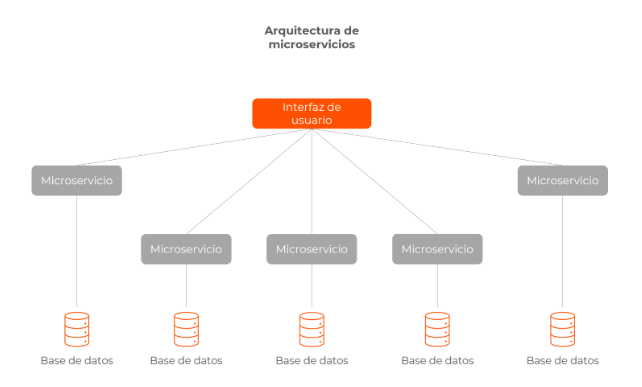
\includegraphics[width=\textwidth]{microservicios}
	\caption{Modelo de arquitectura basada en microservicios}
	\label{fig:microservicios}
\end{figure}

La arquitectura de microservicios funciona como un conjunto de pequeños servicios que se ejecutan de manera independiente y autónoma, es un método de desarrollo de aplicaciones software. En ella, cada microservicio desempeña una función específica y se comunica con el resto a través de APIs, además cuentan con sistemas de almacenamiento propio, lo que evita la sobrecarga y caída de la aplicación.

Los microservicios se encuentran distribuidos y tienen un nivel de acoplamiento bajo, para no influir en los demás. El objetivo es distribuir un software de calidad con mayor rapidez. Puede desarrollar múltiples microservicios de forma simultánea, sin necesidad de volver a diseñar o implementar toda la aplicación después de realizar modificaciones, ya que los servicios se implementan de forma independiente. 

Gracias a ello, varios desarrolladores pueden trabajar en sus servicios individuales al mismo tiempo, en lugar de actualizar toda la aplicación, lo que reduce el tiempo de desarrollo y permite lanzar características nuevas con mayor frecuencia.

Veamos qué ventajas y desventajas tiene la aplicación de una arquitectura de microservicios frente a otros tipos de arquitectura:

\subsubsection{Ventajas}
\begin{itemize}
	\item Modularidad: al tratarse de servicios autónomos, se pueden desarrollar y desplegar de forma independiente. Además un error en un servicio no debería afectar la capacidad de otros servicios para seguir trabajando según lo previsto.
	\item Escalabilidad: como es una aplicación modular, se puede escalar horizontalmente cada parte según sea necesario, aumentando el escalado de los módulos que tengan un procesamiento más intensivo.
	\item Versatilidad: se pueden usar diferentes tecnologías y lenguajes de programación. Lo que permite adaptar cada funcionalidad a la tecnología más adecuada y rentable.
	\item Mantenimiento simple y barato: al poder hacerse mejoras de un solo módulo y no tener que intervenir en toda la estructura, el mantenimiento es más sencillo y barato que en otras arquitecturas.
	\item Rapidez de actuación: el reducido tamaño de los microservicios permite un desarrollo menos costoso, así como el uso de Dockers permite que el despliegue de la aplicación se pueda llevar a cabo rápidamente.
\end{itemize}

\subsubsection{Desventajas}
\begin{itemize}
	\item Coste de implantación alto: una arquitectura de microservicios puede suponer un alto coste de implantación debido a costes de infraestructura y pruebas distribuidas.
	\item Complejidad en la gestión: si contamos con un gran número de microservicios, será más complicado controlar la gestión e integración de los mismos. Es necesario disponer de una centralización de trazas y herramientas avanzadas de procesamiento de información que permitan tener una visión general de todos los microservicios.
	\item Inversión de tiempo inicial: al crear la arquitectura, se necesita más tiempo para poder fragmentar los distintos microservicios e implementar la comunicación entre ellos.
	\item Alto consumo de memoria: al tener cada microservicio sus propios recursos y bases de datos, consumen más memoria y CPU.
\end{itemize}

Podemos nombrar algunos ejemplos de aplicaciones actuales que utilizan este tipo de arquitectura:
\begin{itemize}
	\item Netflix. Esta plataforma tiene una arquitectura generalizada que desde hace ya un par de años se pasó a los microservicios para el funcionamiento de sus productos.
	\item Amazon. No soporta tantos dispositivos como Netflix, pero tampoco es que sea fundamental para cubrir su sector. Migró hace tres años a la arquitectura de microservicios siendo una de las primeras grandes compañías que la implementaban en producción.
\end{itemize}

Tanto la \autoref{fig:microservicios} como la información sobre las arquitecturas de microservicios está sacada de \cite{microservicios}.

\subsection{REST y RESTful}
REST (Representational State Transfer) es un conjunto de criterios de diseño para desarrollar proyectos basados en recursos, que cambió por completo la ingeniería del software y es un concepto fundamental para el desarrollo de cualquier sistema (aplicaciones móviles, sistemas industriales, empresas, negocios, etc...).
\begin{figure}[h!]
	\centering
	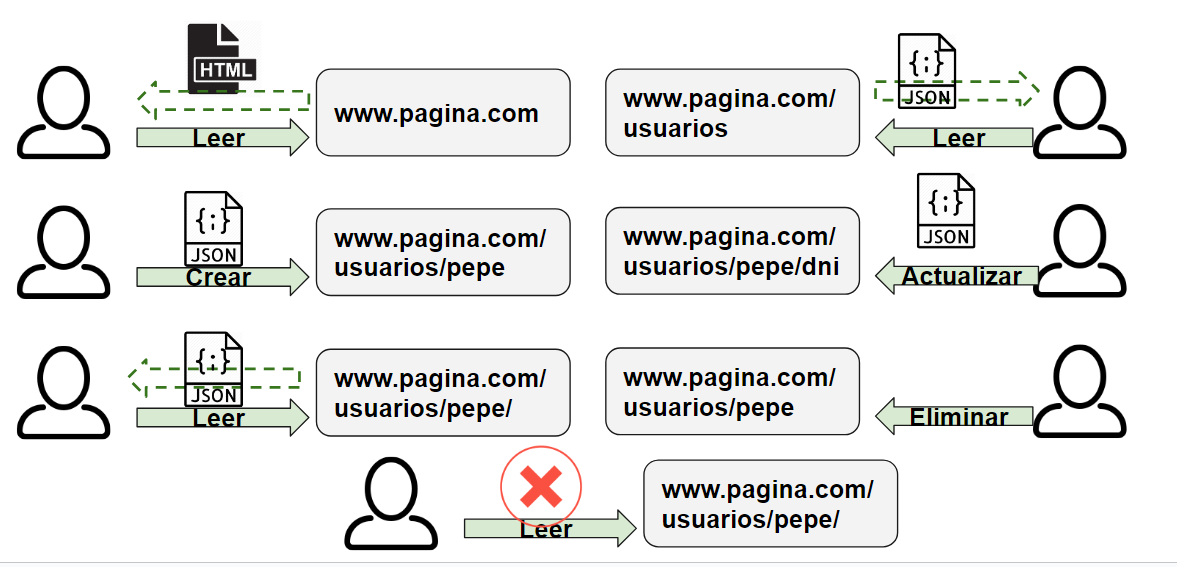
\includegraphics[width=0.9\textwidth]{rest}
	\caption{Ejemplo de las operaciones de transferencia de estado}
	\label{fig:operaciones}
\end{figure} RESTful se suele utilizar para referirse a los servicios web de ejecución de una arquitectura REST.
El objetivo de REST es definir recursos, modificarlos e intercambiar la representación de estos en un formato concreto: XML, JSON, HTML, texto plano, etc... Estos recursos se identifican de forma única mediante un URI \textit{(Uniform Resource Identifier)} y son accesibles globalmente, además se construyen de forma dinámica. Estos recursos se pueden manipular a través de operaciones estándar de HTTP como pueden ser GET, POST, PUT o DELETE que sirven para leer, actualizar, crear y eliminar, respectivamente.
En la \autoref{fig:operaciones} podemos ver un ejemplo de uso de las distintas operaciones.

Los recursos se pueden clasificar en dos tipos principalmente:
\begin{itemize}
	\item Entrypoint: URL de un sitio web para visualizar el contenido, están diseñados para interactuar con el usuario final.
	\item Endpoint: URL de una API que responde a una petición, a diferencia del entrypoint, no están diseñados para interactuar con el usuario final.
\end{itemize}
Las principales ventajas que nos ofrece el uso de REST son:
\begin{itemize}
	\item Separación entre cliente y servidor que nos permite distinguir entre la interfaz de usuario del servidor y del almacenamiento de datos, además de mejorar la portabilidad con otros proyectos.
	\item Visibilidad, fiabilidad y escalabilidad gracias a la separación entre cliente y servidor añadiendo nuevos recursos.
	\item El desarrollo orientado a recursos es muy modular, al usar encapsulación y reusabilidad.
	\item La interfaz de acceso a los diferentes recursos es universal, debido al uso de HTTP, JSON/XML y ser independiente de cualquier plataforma.
	\item Es uno de los conceptos más ampliamente usados actualmente para el desarrollo, prácticamente cualquier sistema actual usa tecnología REST/RESTful en su backend.
\end{itemize}
Sin embargo, también existen algunas desventajas:
\begin{itemize}
	\item Es necesario abordar problemas de una forma distinta, cambiando el modo de pensar.
	\item Al principio requiere un mayor tiempo de desarrollo y más conocimientos que otros modelos clásicos de servicios web.
\end{itemize}

La información acerca de la arquitectura REST está basada principalmente en \cite{restful}.

\section{Tecnologías Backend}
Hemos implementado la API utilizando Python y Flask, pero otra opción hubiera sido con Java y Spring, a continuación mostramos una comparación exhaustiva entre ambos:

Flask y Spring son ambos populares frameworks web que permiten construir aplicaciones web. Sin embargo, hay varias diferencias clave entre ellos en cuanto a su arquitectura, enfoque de desarrollo y uso.
\begin{itemize}
	\item Estructura: Flask es un micro-framework, mientras que Spring es un framework completo. Flask permite a los desarrolladores tener más flexibilidad a la hora de elegir componentes y bibliotecas para construir su aplicación. Por otro lado, Spring viene con una estructura predefinida, proporcionando un enfoque más valorado para el desarrollo web.
	\item Lenguaje: Flask se usa principalmente con Python, mientras que Spring se usa comúnmente con Java. Python es conocido por su simplicidad y legibilidad, lo que hace de Flask una opción popular para proyectos pequeños a medianos. Java, por otro lado, es un lenguaje más versátil y ampliamente utilizado, lo que hace de Spring el framework preferido para aplicaciones a gran escala a nivel empresarial.
	\item Filosofía de Desarrollo: Flask sigue la filosofía de "Do-it-yourself", donde los desarrolladores tienen más control sobre el proceso de desarrollo. Permite a los desarrolladores elegir e integrar varios componentes según sus requisitos. Spring, por otro lado, sigue la filosofía de "Convention over Configuration", proporcionando un conjunto de configuraciones y convenciones predefinidas para simplificar el desarrollo. Esto puede acelerar el desarrollo pero puede limitar la flexibilidad.
	\item Comunidad y Ecosistema: Flask tiene una comunidad más pequeña en comparación con Spring, pero es altamente activa y está creciendo rápidamente, además, cuenta con una amplia gama de extensiones y bibliotecas de terceros, lo que facilita encontrar soluciones para necesidades específicas. Spring, por otro lado, tiene una comunidad más grande y madura con una extensa documentación y soporte.
	\item Curva de Aprendizaje: Flask tiene una curva de aprendizaje relativamente baja debido a su simplicidad y enfoque minimalista. Es fácil comenzar con Flask y construir una aplicación básica rápidamente. Spring, por otro lado, tiene una curva de aprendizaje más pronunciada debido a sus características extensas y complejidad. Requiere una comprensión más profunda de Java y Spring.
	\item Adecuación: Flask es adecuado para aplicaciones pequeñas y medianas, prototipos y desarrollo rápido. Es ideal para proyectos que requieren flexibilidad y soluciones personalizadas. Spring, por otro lado, es más adecuado para aplicaciones a nivel empresarial a gran escala con requisitos complejos. Proporciona un amplio soporte para seguridad, escalabilidad e integración con otros sistemas empresariales.
\end{itemize}

En resumen, Flask y Spring difieren en cuanto a su estructura, lenguaje, filosofía de desarrollo, soporte comunitario, curva de aprendizaje y adecuación para diferentes tamaños de proyecto. Flask ofrece más flexibilidad y simplicidad, mientras que Spring proporciona un marco integral con amplias características a nivel empresarial.
\section{Tecnologías Frontend}
Para el desarrollo del Frontend de nuestro proyecto, nos hemos decidido por React, una biblioteca de JavaScript muy popular. Sin embargo, es importante mencionar que Angular también fue considerado como una opción viable debido a sus similitudes con React.

\subsection{React vs. Angular}
React se destaca por su enfoque minimalista, lo que lo hace relativamente fácil de entender para aquellos familiarizados con JavaScript. Sin embargo, configurar un proyecto en React puede llevar tiempo, y el dominio de librerías adicionales es necesario para gestionar el estado de la aplicación. Además, las actualizaciones frecuentes de React requieren un esfuerzo adicional por parte del desarrollador para mantenerse al día con las mejores prácticas y cambios en la sintaxis.\\

Angular, por otro lado, presenta una curva de aprendizaje más pronunciada debido a su gran tamaño y complejidad. Aunque TypeScript, el lenguaje en el que está basado Angular, se asemeja a JavaScript, aprender todos los conceptos asociados con Angular lleva más tiempo. Además, las actualizaciones constantes de Angular requieren un esfuerzo adicional de aprendizaje por parte del desarrollador.\\

Si bien React cuenta con una gran comunidad de desarrolladores que respaldan su continuo desarrollo, Angular presenta cierto rechazo debido a su complejidad percibida, especialmente después de la versión 1.0, que no tuvo mucho éxito. Sin embargo, el respaldo de Google ha mejorado la credibilidad de Angular, y su uso por parte de grandes empresas como McDonald's y Apple subraya su relevancia en la industria.\\

React ofrece a los desarrolladores la libertad de elegir la estructura de su aplicación, lo que se convierte en una mayor flexibilidad, pero también en una mayor complejidad al inicio del proyecto. Por otro lado, Angular proporciona una estructura fija y compleja, más adecuada para desarrolladores experimentados. Su arquitectura basada en tres capas (modelo, controlador y vista), implica una mayor formalidad en la organización del código.\\

En resumen, la elección entre React y Angular depende de las necesidades y preferencias del proyecto, considerando factores como la curva de aprendizaje, la comunidad de soporte y la estructura deseada para la aplicación. Ambos tienen sus ventajas y desventajas, y la elección final dependerá de los objetivos y requisitos específicos de desarrollo.

\endinput
%------------------------------------------------------------------------------------
% FIN DEL CAPÍTULO. 
%----------------------------------------------------------------------------------
-